\documentclass[border=4pt]{standalone}
\usepackage[T1]{fontenc}
\usepackage{tikz}
\usetikzlibrary{arrows.meta,positioning,fit,backgrounds,shapes.geometric,calc}
\definecolor{orch}{HTML}{234767}
\definecolor{ctx}{HTML}{EAF1F8}
\definecolor{retr}{HTML}{E2F0ED}
\definecolor{ext}{HTML}{F7EBDD}
\definecolor{infra}{HTML}{F1F3F5}
\tikzset{
 every node/.style={font=\sffamily\fontsize{8.5}{10}\selectfont,align=center,execute at begin node={\hyphenpenalty=10000\exhyphenpenalty=10000}},
 block/.style={draw=orch!80,fill=white,rounded corners=1.5pt,minimum height=7mm,inner sep=3pt,line width=.55pt},
 context/.style={block,fill=ctx},
 engine/.style={block,fill=orch,text=white},
 retrieval/.style={block,fill=retr},
 external/.style={block,fill=ext},
 storage/.style={block,fill=infra},
 optional/.style={dashed},
 flow/.style={-{Stealth[length=2mm]},draw=orch!90,line width=.65pt},
 control/.style={flow,dashed},
 error/.style={flow,densely dotted},
 group/.style={draw=orch!50,rounded corners=3pt,inner sep=5pt,line width=.5pt},
 heading/.style={font=\sffamily\bfseries\fontsize{8.5}{10}\selectfont,text=orch},
 edgelabel/.style={font=\sffamily\fontsize{7.5}{9}\selectfont,fill=white,inner sep=1pt,text=orch}
}

\begin{document}
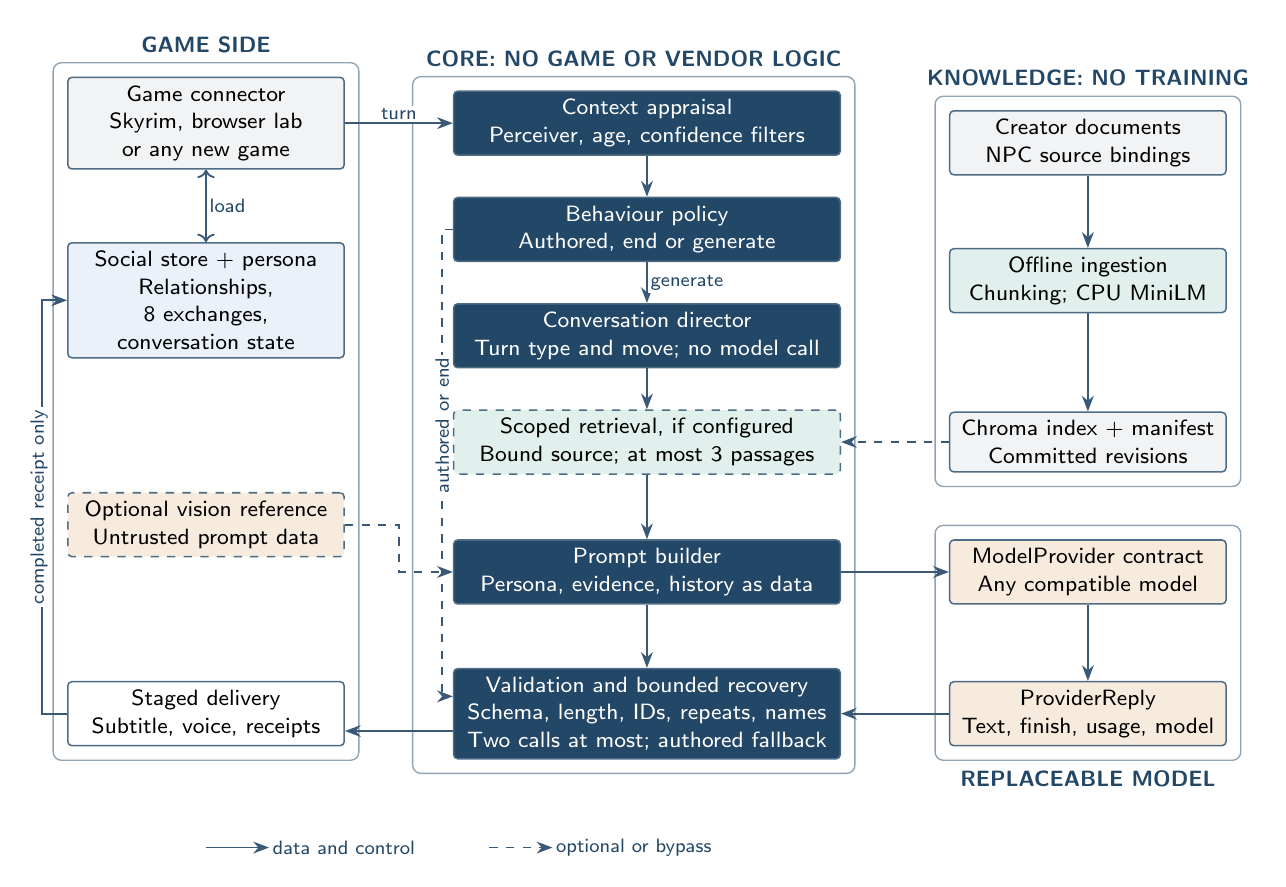
\begin{tikzpicture}
% Connector column
\node[storage,text width=3.3cm] (game) at (0,8) {Game connector\\Skyrim, browser lab or any new game};
\node[context,text width=3.3cm] (store) at (0,5.75) {Social store + persona\\Relationships, 8 exchanges, conversation state};
\node[external,optional,text width=3.3cm] (cv) at (0,2.9) {Optional vision reference\\Untrusted prompt data};
\node[block,text width=3.3cm] (out) at (0,.5) {Staged delivery\\Subtitle, voice, receipts};
% Core chain
\node[engine,text width=4.7cm] (ctx) at (5.6,8) {Context appraisal\\Perceiver, age, confidence filters};
\node[engine,text width=4.7cm] (pol) at (5.6,6.65) {Behaviour policy\\Authored, end or generate};
\node[engine,text width=4.7cm] (dir) at (5.6,5.3) {Conversation director\\Turn type and move; no model call};
\node[retrieval,optional,text width=4.7cm] (ret) at (5.6,3.95) {Scoped retrieval, if configured\\Bound source; at most 3 passages};
\node[engine,text width=4.7cm] (pro) at (5.6,2.3) {Prompt builder\\Persona, evidence, history as data};
\node[engine,text width=4.7cm] (val) at (5.6,.5) {Validation and bounded recovery\\Schema, length, IDs, repeats, names\\Two calls at most; authored fallback};
% Right column
\node[storage,text width=3.3cm] (docs) at (11.2,7.75) {Creator documents\\NPC source bindings};
\node[retrieval,text width=3.3cm] (ing) at (11.2,6) {Offline ingestion\\Chunking; CPU MiniLM};
\node[storage,text width=3.3cm] (idx) at (11.2,3.95) {Chroma index + manifest\\Committed revisions};
\node[external,text width=3.3cm] (prov) at (11.2,2.3) {ModelProvider contract\\Any compatible model};
\node[external,text width=3.3cm] (rep) at (11.2,.5) {ProviderReply\\Text, finish, usage, model};
% Core flow
\draw[flow] (game) -- node[edgelabel,above]{turn} (ctx);
\draw[flow] (ctx) -- (pol);
\draw[flow] (pol) -- node[edgelabel,right]{generate} (dir);
\draw[flow] (dir) -- (ret);
\draw[flow] (ret) -- (pro);
\draw[flow] (pro) -- (val);
\draw[control] (pol.west) -- (3.0,6.65) -- node[edgelabel,pos=.42,rotate=90]{authored or end} (3.0,.72) -- ($(val.west)+(0,.22)$);
% Connector and memory
\draw[flow,<->] (game) -- node[edgelabel,right]{load} (store);
\draw[flow] ($(val.west)+(0,-.22)$) -- ($(out.east)+(0,-.22)$);
\draw[flow] (out.west) -- ++(-.32,0) |- node[edgelabel,pos=.25,rotate=90,yshift=1pt]{completed receipt only} (store.west);
\draw[control] (cv.east) -- (2.45,2.9) |- (pro.west);
% Knowledge and model
\draw[flow] (docs) -- (ing);
\draw[flow] (ing) -- (idx);
\draw[control] (idx) -- (ret);
\draw[flow] (pro) -- (prov);
\draw[flow] (prov) -- (rep);
\draw[flow] (rep) -- (val);
\begin{pgfonlayer}{background}
\node[group,fit=(game)(store)(cv)(out),label={[heading]above:GAME SIDE}] {};
\node[group,fit={(ctx)(val)(2.8,8)},label={[heading]above:{CORE: NO GAME OR VENDOR LOGIC}}] {};
\node[group,fit=(docs)(ing)(idx),label={[heading]above:{KNOWLEDGE: NO TRAINING}}] {};
\node[group,fit=(prov)(rep),label={[heading]below:REPLACEABLE MODEL}] {};
\end{pgfonlayer}
\draw[flow] (0,-1.2) -- (.8,-1.2) node[edgelabel,right] {data and control};
\draw[control] (3.6,-1.2) -- (4.4,-1.2) node[edgelabel,right] {optional or bypass};
\end{tikzpicture}
\end{document}
